\documentclass{article}

\usepackage[utf8]{inputenc}
\usepackage[margin=0.75in]{geometry}
\usepackage{amsmath, amssymb}
\usepackage{graphicx}
\usepackage{hyperref}
\usepackage{url}

\graphicspath{{./images}}

\begin{document}

\title{Security \& Privacy of Machine Learning --- Assignment 3 Write-Up}
\author{Daan Brugmans (S1080742)}
\date{\today}

\maketitle

My Jupyter notebook and report can also be found publicly on GitHub \href{https://github.com/daanbrugmans/ru-security-and-privacy-of-machine-learning-23-24/tree/main/assignments/assignment-3}{at this URL.}
My implementation of the assignment consists of two parts: the setup, which contains all implementations of everything I need in order to answer the assignment questions, and the assignment questions themselves.
I will adhere to this structure for this write-up as well.

\section{Setup}
\subsection{Imports, Preparation, and Metrics}
I use PyTorch as the main environment for building and training a deep learning model, since that is the deep learning framework I am most comfortable with. 
At the start of the notebook, I execute some preparatory code.
I set a seed for \textit{torch}, \textit{NumPy}, and Python itself for improved reproducibility, and I also include a function for visualizing the $L_2$-norm of model state dicts.
I include an implementation for the Attack Success Rate as a metric.

\subsection{Data}
For loading the data, I have implemented a function that automatically loads the CIFAR-10 dataset and returns dataloaders for a train, validation, and test set.

\subsection{Model}
The class \texttt{NeuralModel} is a collection of all processes and objects that are needed for training a neural network.
It contains an instance of the pre-trained \texttt{ResNet18Light} network, its loss function, its optimizer, the number of training epochs, and dataloaders for the train, validation, and test sets.
I have chosen to implement it this way, so that all code related to the neural network and its architecture is encapsulated within a single class.
In my opinion, this makes performing varying attacks very clean: with only a few rows of code, I am able to instantiate, train, and test a new model.
This makes the experiments easy to read and hides away set implementation details.

\subsection{Attacks and Defenses}
I define classes for \href{https://arxiv.org/abs/1708.06733}{BadNet Attacks} and \href{https://arxiv.org/pdf/1712.05526}{Blend Attacks}, in addition to functions for the \href{http://proceedings.mlr.press/v108/bagdasaryan20a/bagdasaryan20a.pdf}{Scaling Attack and Clipping Defense}.
I made the implementation for the Blend Attack myself, using template code from the week 8 tutorial.
I also made the implementation for the clipping function myself, while the scaling attack code comes from the tutorial on Federated Learning.
For the BadNet Attack, I have implemented versions for regular and a distributed attack.
The implementation for the regular version uses existing functionality from \texttt{src}, but for the distributed version, I added the new functionality myself.
This new functionality is incorporated into the existing codebase, meaning that some code in \texttt{src} has been altered.

\subsection{Federated Learning}
For the code regarding Federated Learning (FL), dr. Picek has provided a library that implements a fully functioning FL environment.
I make use of this code and it is found in the \texttt{src} folder.
I use this code to set up an FL environment.
The \texttt{FLSettings} class consists of a collection of variables that we use throughout the codebase to tweak FL settings, such as the number of malignant clients or which aggregation function to use.
To simulate an FL scenario, I define a collection of code blocks.
I define a single function called \texttt{learn\_federated} that executes an entire FL scenario with a single function call.
I also define the different aggregation functions that we will use (FedAvg and Krum) and use the code in \texttt{src} to setup an FL environment.

\section{Assignment Questions}
% \begin{table}
%     \centering
%     \begin{tabular}{cols}
        
%     \end{tabular}
%     \caption{}
%     \label{tab:}
% \end{table}

% \begin{figure}
%     \centering
%     \includegraphics[width=0.9\textwidth]{}
%     \caption{}
%     \label{fig:}
% \end{figure}

\subsection{Backdoor Attack in Federated Learning}
\subsubsection{Implement a source-agnostic backdoor attack in FL using the
Blend attack with the Hello Kitty image. Below you find a list of parameters/settings to use for this attack. Limit your implementation to these values.
You will be investigating the performance of the attack with different number of
malicious clients in the network, i.e., 1, 2, or 3. In all cases, a total of 6 clients
compose the network. For example, in the first setting you have 1 malicious
and 5 benign clients. However, we ask you to select only a subset from all the
clients each round to perform the local training. This subset selection should be
random, but you are free how you implement this selection procedure. In the
end of the training, i.e., after 5 rounds of FL, plot the final ASR (y-axis) and
the global (poisoned) model’s task accuracy (also y-axis) versus the number of
malicious clients (x-axis). Either make two plots, one for ASR and one for accuracy, or combine the results in one. The following parameters/settings should
be used:}
\begin{itemize}
    \item \textbf{Model}: Load the pre-trained ResNet18Light model from the Federated
    Learning tutorial.
    \item \textbf{Poisoning Rate}: Every malicious client should use a poisoning rate of
    50\% of the local dataset.
    \item \textbf{Global Aggregation Rounds}: 5
    \item \textbf{Local Training Epochs}: 2
    \item \textbf{Backdoor Target Class}: 0 (airplane)
    \item \textbf{Number Selected Clients Per Round}: 5
    \item \textbf{Aggregation Method}: FedAvg
\end{itemize}

\begin{figure}[h]
    \centering
    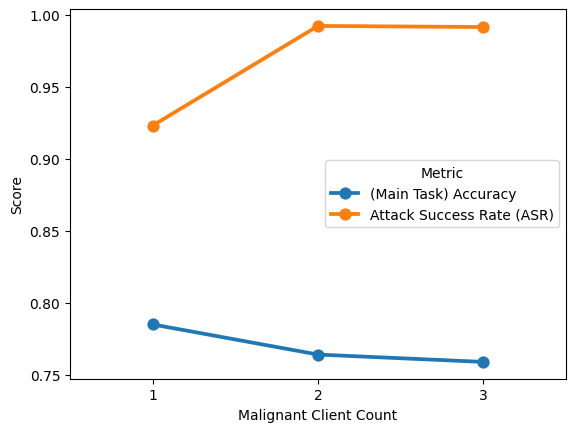
\includegraphics[width=0.5\textwidth]{malignant_client_count.png}
    \caption{The Main Task Accuracy and Attack Success Rate of the global model with a varying amount of malignant clients.}
    \label{fig:malignant_client_count}
\end{figure}

See figure \ref{fig:malignant_client_count}.

\subsubsection{In question 1(a) we asked you to use a subset of clients each round.
What do you think is the influence of the number of selected clients on the
performance of the backdoor attack in the federated setting? Share your conclusions.}
I think that the influence of the number of selected clients on the performance of the backdoor attack will vary significantly depending on what we assume that the share of malignant clients will be.
If the share of malignant clients is small, then I expect the procedure to be a mildly useful defense, as the global model has an opportunity to recuperate from learning the backdoor every once in a while when a malignant user is excluded.
However, if the share of malignant clients is bigger, or even approaching a 50/50 split between benign and malignant clients, then I think that the procedure may only make the backdoor more effective, since there is a real chance that there will be rounds where the global model aggregates from mostly or exclusively malignant clients.
This dynamic holds true for when the number of selected clients changes: the smaller the number of selected clients is, the more likely it is that the model aggregates from mostly malignant clients for some rounds, and the more likely it is that the backdoor will be inserted.

\subsubsection{In question 1(a) we asked you to perform Federated Learning using
the FedAvg method for aggregation. Now using the same settings, but with just
1 malicious client, perform federated learning by making use of the Krum aggregation method. Plot the final ASR (y-axis) and global (poisoned) model task
accuracy (y-axis) for both the FedAvg and Krum methods (x-axis). Compare
the methods and share your conclusions on how both methods affect the ASR
and accuracy. For this homework question we ask you to assume 1 malicious
client, so f = 1. Also, only consider the subset of local models each round for
aggregation.}
\begin{figure}
    \centering
    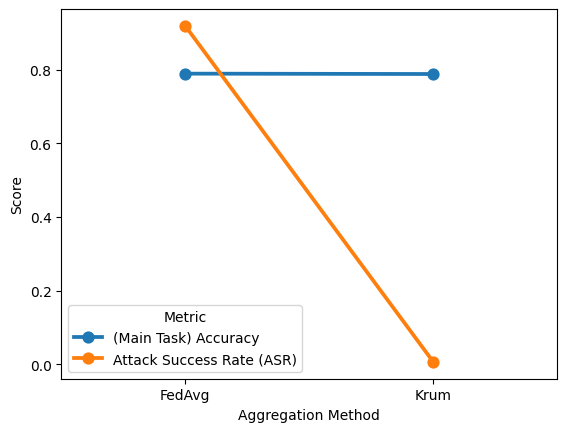
\includegraphics[width=0.5\textwidth]{aggregation_method.png}
    \caption{The Main Task Accuracy and Attack Success Rate of the global model with a varying aggregation methods.}
    \label{fig:aggregation_method}
\end{figure}

When Krum aggregates the weights, it chooses only a subset of the local models to update the global model.
It chooses this subset by calculating the Euclidean distances between the local models' weights.
Benign models will be close to each other in the Euclidean weight space, since they were trained on similar, unaltered data.
Malignant models will be further removed from other models, since they were trained on data that was altered.
Having learned from altered data, the weights of the malignant models will look more different from each other and from the benign models than the weights from benign models will look from other benign models.
By comparing these weights using the Euclidean distance, we find the models whose weights are most similar to one another, since they were trained on similar data, and Krum then picks these models to aggregate local weights from.
This way, Krum excludes local models which are further removed from other models in the Euclidean space, which are likely to be malignant/backdoored.

In figure \ref{fig:aggregation_method}, we can see that the accuracy for the global models is nearly identical when using either FedAvg or Krum.
However, while FedAvg results in a model with an ASR of over 90\%, the ASR drops to near-zero when Krum is used as an aggregation method.
This is because of the reason explained above: Krum excludes the malignant model from the aggregation process by recognizing that it is far removed from the benign models in a Euclidean space.
The malignant model's exclusion from the aggregation prevents the insertion of the backdoor, which is why the ASR is so low when using Krum.
FedAvg does not have a check for potentially malignant models, so they are always included in the aggregation, meaning that the backdoor will be learned by the model with every aggregation round.

\subsection{Distributed Backdoor Attack}
\subsubsection{Implement the Distributed Backdoor Attack (DBA). The network
of clients is composed of three malicious clients and three benign clients. The
three malicious clients will split a red 6 x 6 square trigger vertically into three
equal parts. Use the following parameters/settings for your attack: (see list below)
Plot the final ASR (y-axis) and global (poisoned) model task accuracy (y-axis).
Compare your results with your plot from question 1(a). How does DBA perform
compared to the previous FL attack setting? Which FL attack setup performs
best and why do you think this is the case? Share your conclusions.}
\begin{itemize}
    \item \textbf{Model}: Load the pre-trained ResNet18Light model from the Federated
    Learning tutorial.
    \item \textbf{Poisoning Rate}: Every malicious client should use a poisoning rate of
    50\% of the local dataset.
    \item \textbf{Global Aggregation Rounds}: 5
    \item \textbf{Local Training Epochs}: 2
    \item \textbf{Backdoor Target Class}: 0 (airplane)
    \item \textbf{Number Selected Clients Per Round}: 6
    \item \textbf{Aggregation Method}: FedAvg
\end{itemize}

\begin{figure}
    \centering
    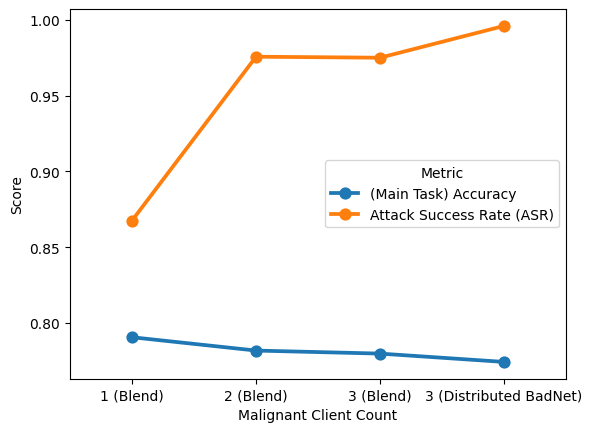
\includegraphics[width=0.5\textwidth]{dba.png}
    \caption{The Main Task Accuracy and Attack Success Rate of the global model with either 1, 2, or 3 malignant clients that attack the model independently, or 3 malignant clients that coordinate a distributed attack together.}
    \label{fig:dba}
\end{figure}

Figure \ref{fig:dba} shows the ASR and accuracy of the global model after an FL scenario with 1, 2, or 3 malignant users who independently used a Blend attack, and of the global model after an FL scenario with 3 malignant users who coordinated a distributed BadNet attack.
As we can see, the distributed attack is even more successful than all the Blend attacks, attaining an ASR of 0.996; a practically perfect backdoor.
This has come at the cost of a very slight accuracy drop.

I think that the success of the distributed BadNet attack comes from the fact that the malignant clients have turned the singular trigger into a collection of multiple smaller triggers, which are all learned by the model as independent features.
Over multiple aggregation rounds, both the global and local models learn to associate every malignant client's local trigger individually.
In our example, the models learn that a red column at any of the three regions in the image where a backdoor can be inserted is a feature of the target class.
This implies that the models see the individual malignant clients' triggers as independent features to learn.
Once training has finished, and the model is used for inference, it receives an image with the full trigger.
When it receives such an image, it is intensely convinced that it is an image of the target class, since the image does not contain just one red column, but it contains all three red columns; the image has all the red column features, of which only one would already indicate that the image belongs to the target class.
Since the image contains all the features associated with the individual malignant clients' triggers, the model will be very sure that the image belongs to the target class, and classifies it as such.
In other words: the model has not learned the trigger as a singular feature, but has learned 3 features that all correspond to $\frac{1}{3}\text{rd}$ of the trigger.

\subsection{Clipping Defense}
For this part you are going to perform the clipping defense, but first you will perform
the scaling attack as explained in the lecture and tutorial. After applying the scale
update to the malicious client and aggregating the results, you will investigate the
effect of the clipping defense.

\subsubsection{Take exactly the same settings as question 1(a) but limit it to just 1
malicious client. Use the blend attack and at each round let the malicious client
apply the scale update with a scaling factor of $\gamma = \frac{n}{\mu}$. Here $n$ is the number of
clients and $\mu$ is the learning rate which is also the number of malicious clients
and thus now set to 1. Finally, plot the ASR (y-axis) and global model accuracy
(y-axis) for just the “scaling approach” (x-axis). Store these results, as you will
reuse them in a new plot for the next question.}
\begin{figure}
    \centering
    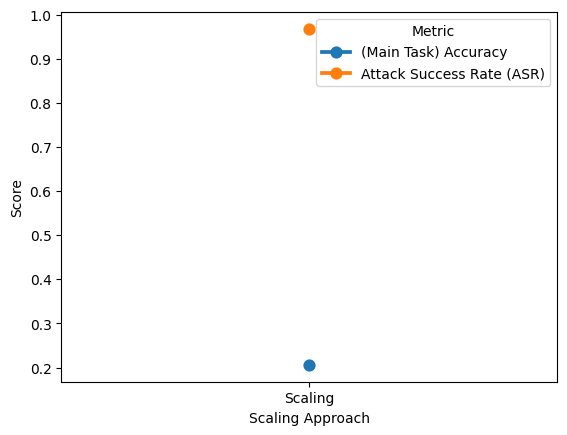
\includegraphics[width=0.5\textwidth]{scaling_attack.png}
    \caption{The Main Task Accuracy and Attack Success Rate of the global model with a malignant user that used a scaled Blend attack.}
    \label{fig:scaling_attack}
\end{figure}

See figure \ref{fig:scaling_attack}.

\subsubsection{Enforce an upper boundary for the $L_2$-norms of model updates, restricting the Euclidean distances between the global and the respective local
models. The model shall be down-scaled if the $L_2$-norm exceeds the boundary (clipping).}
See figure \ref{fig:clipping_defense} for the accuracy and ASR, figure \ref{fig:before_clipping} for the $L_2$-norms before clipping, and figure \ref{fig:after_clipping} for the $L_2$-norms after clipping.


From the results shown in figure \ref{fig:clipping_defense}, I would consider the defense to be ineffective.
Regardless of clipping being applied as a defense, the scaling attack succeeds at inserting a backdoor into the global model.
The clipping defense has barely changed this fact: although the ASR has dropped, it is still high, and the accuracy is still very low.
However, when the logs of the aggregation rounds are inspected, one can see that some rounds end with an accuracy much higher than the final accuracy.
This would imply that the clipping defense does have some effect, but that this effect is too weak to properly mitigate the scaling attack in its entirety.
We can see this in the graphs of figures \ref{fig:before_clipping} and \ref{fig:after_clipping}: the poisoned $L_2$-norm has been clipped, but only very slightly (which may require a zoom-in to see well), and is still much larger than the benign $L_2$ norms.

\section{Quality Discussion}
I would argue that the quality of my results are good enough to showcase the varying FL scenarios and how they differ from one another.
We can easily interpret the effects of how the number of malignant clients influences the global model's ability to learn the backdoor, how different aggregation methods influence this ability to learn the backdoor, how distributing an attack influences the ability to learn the backdoor, how the scaling attack affects the global model, and how the clipping defense mitigates the scaling attack.
I was able to achieve this level of quality by making use of both the code that I had already written for assignment 2 and the code provided by the lecturers in the \texttt{src} directory.

\begin{figure}[h]
    \centering
    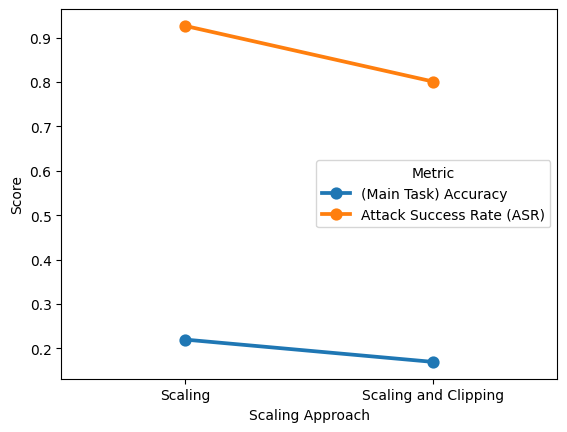
\includegraphics[width=0.5\textwidth]{clipping_defense.png}
    \caption{The Main Task Accuracy and Attack Success Rate of the global model with a clipping defense.}
    \label{fig:clipping_defense}
\end{figure}

\begin{figure}[h]
    \centering
    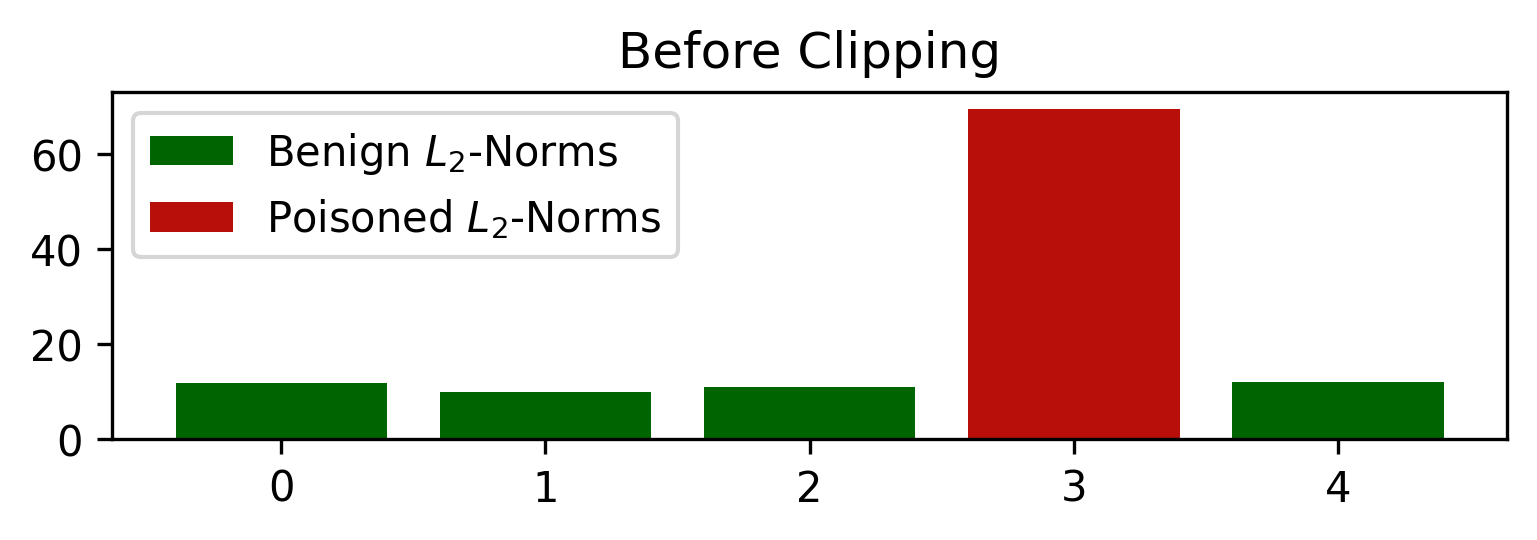
\includegraphics[width=0.6\textwidth]{before_clipping.png}
    \caption{The $L_2$ norms of the local models at the final aggregation round before clipping.}
    \label{fig:before_clipping}
\end{figure}

\begin{figure}[h]
    \centering
    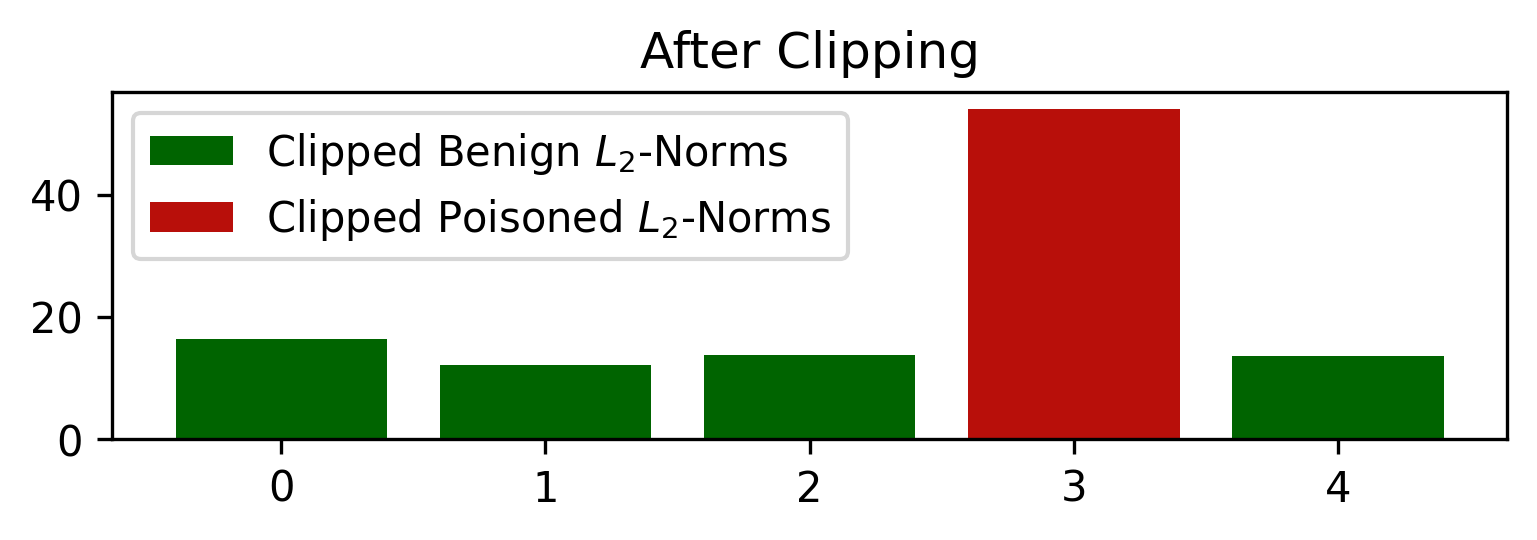
\includegraphics[width=0.6\textwidth]{after_clipping.png}
    \caption{The $L_2$ norms of the local models at the final aggregation round after clipping.}
    \label{fig:after_clipping}
\end{figure}

\end{document}